\section{Auswertung}
\label{sec:Auswertung}

\subsection{Bestimmung der Zeitkonstante $\tau$}

Weil das vom Oszilloskop angezeigte Bild teilweise etwas flackerte, sind zur Aufnahme der Messwerte die in \ref{fig:messA}
gezeigten Fotos aufgenommen worden. 
Hierbei wird durch Abbildung \subref{fig:maxU_C} die Amplitude der Generatorspannung indirekt angezeigt: 
Bei niedriger Frequenz -- hier ${\SI{25.11}{\hertz}}$ -- wird der Kondensator nahezu vollständig geladen und ebenso wieder entladen. 
Somit wird eine Generatorspannung von ${U_0=\SI{4.8}{\volt}}$ abgelesen (gemäß der verwendeten Skalierung entspricht 
ein Kästchen einem Volt). 

In \subref{fig:UpAndDown} beläuft sich eine Periodendauer auf genau vier Kästchen auf der Zeitachse. 
Mit der Frequenz ${f=\SI{244.1}{\hertz}}$ kann eine entsprechende Relation zwischen der Anzahl der Kästchen und der 
Zeit hergestellt werden. 

\begin{figure}
    \centering
    \begin{subfigure}{0.48\textwidth}
        \centering
        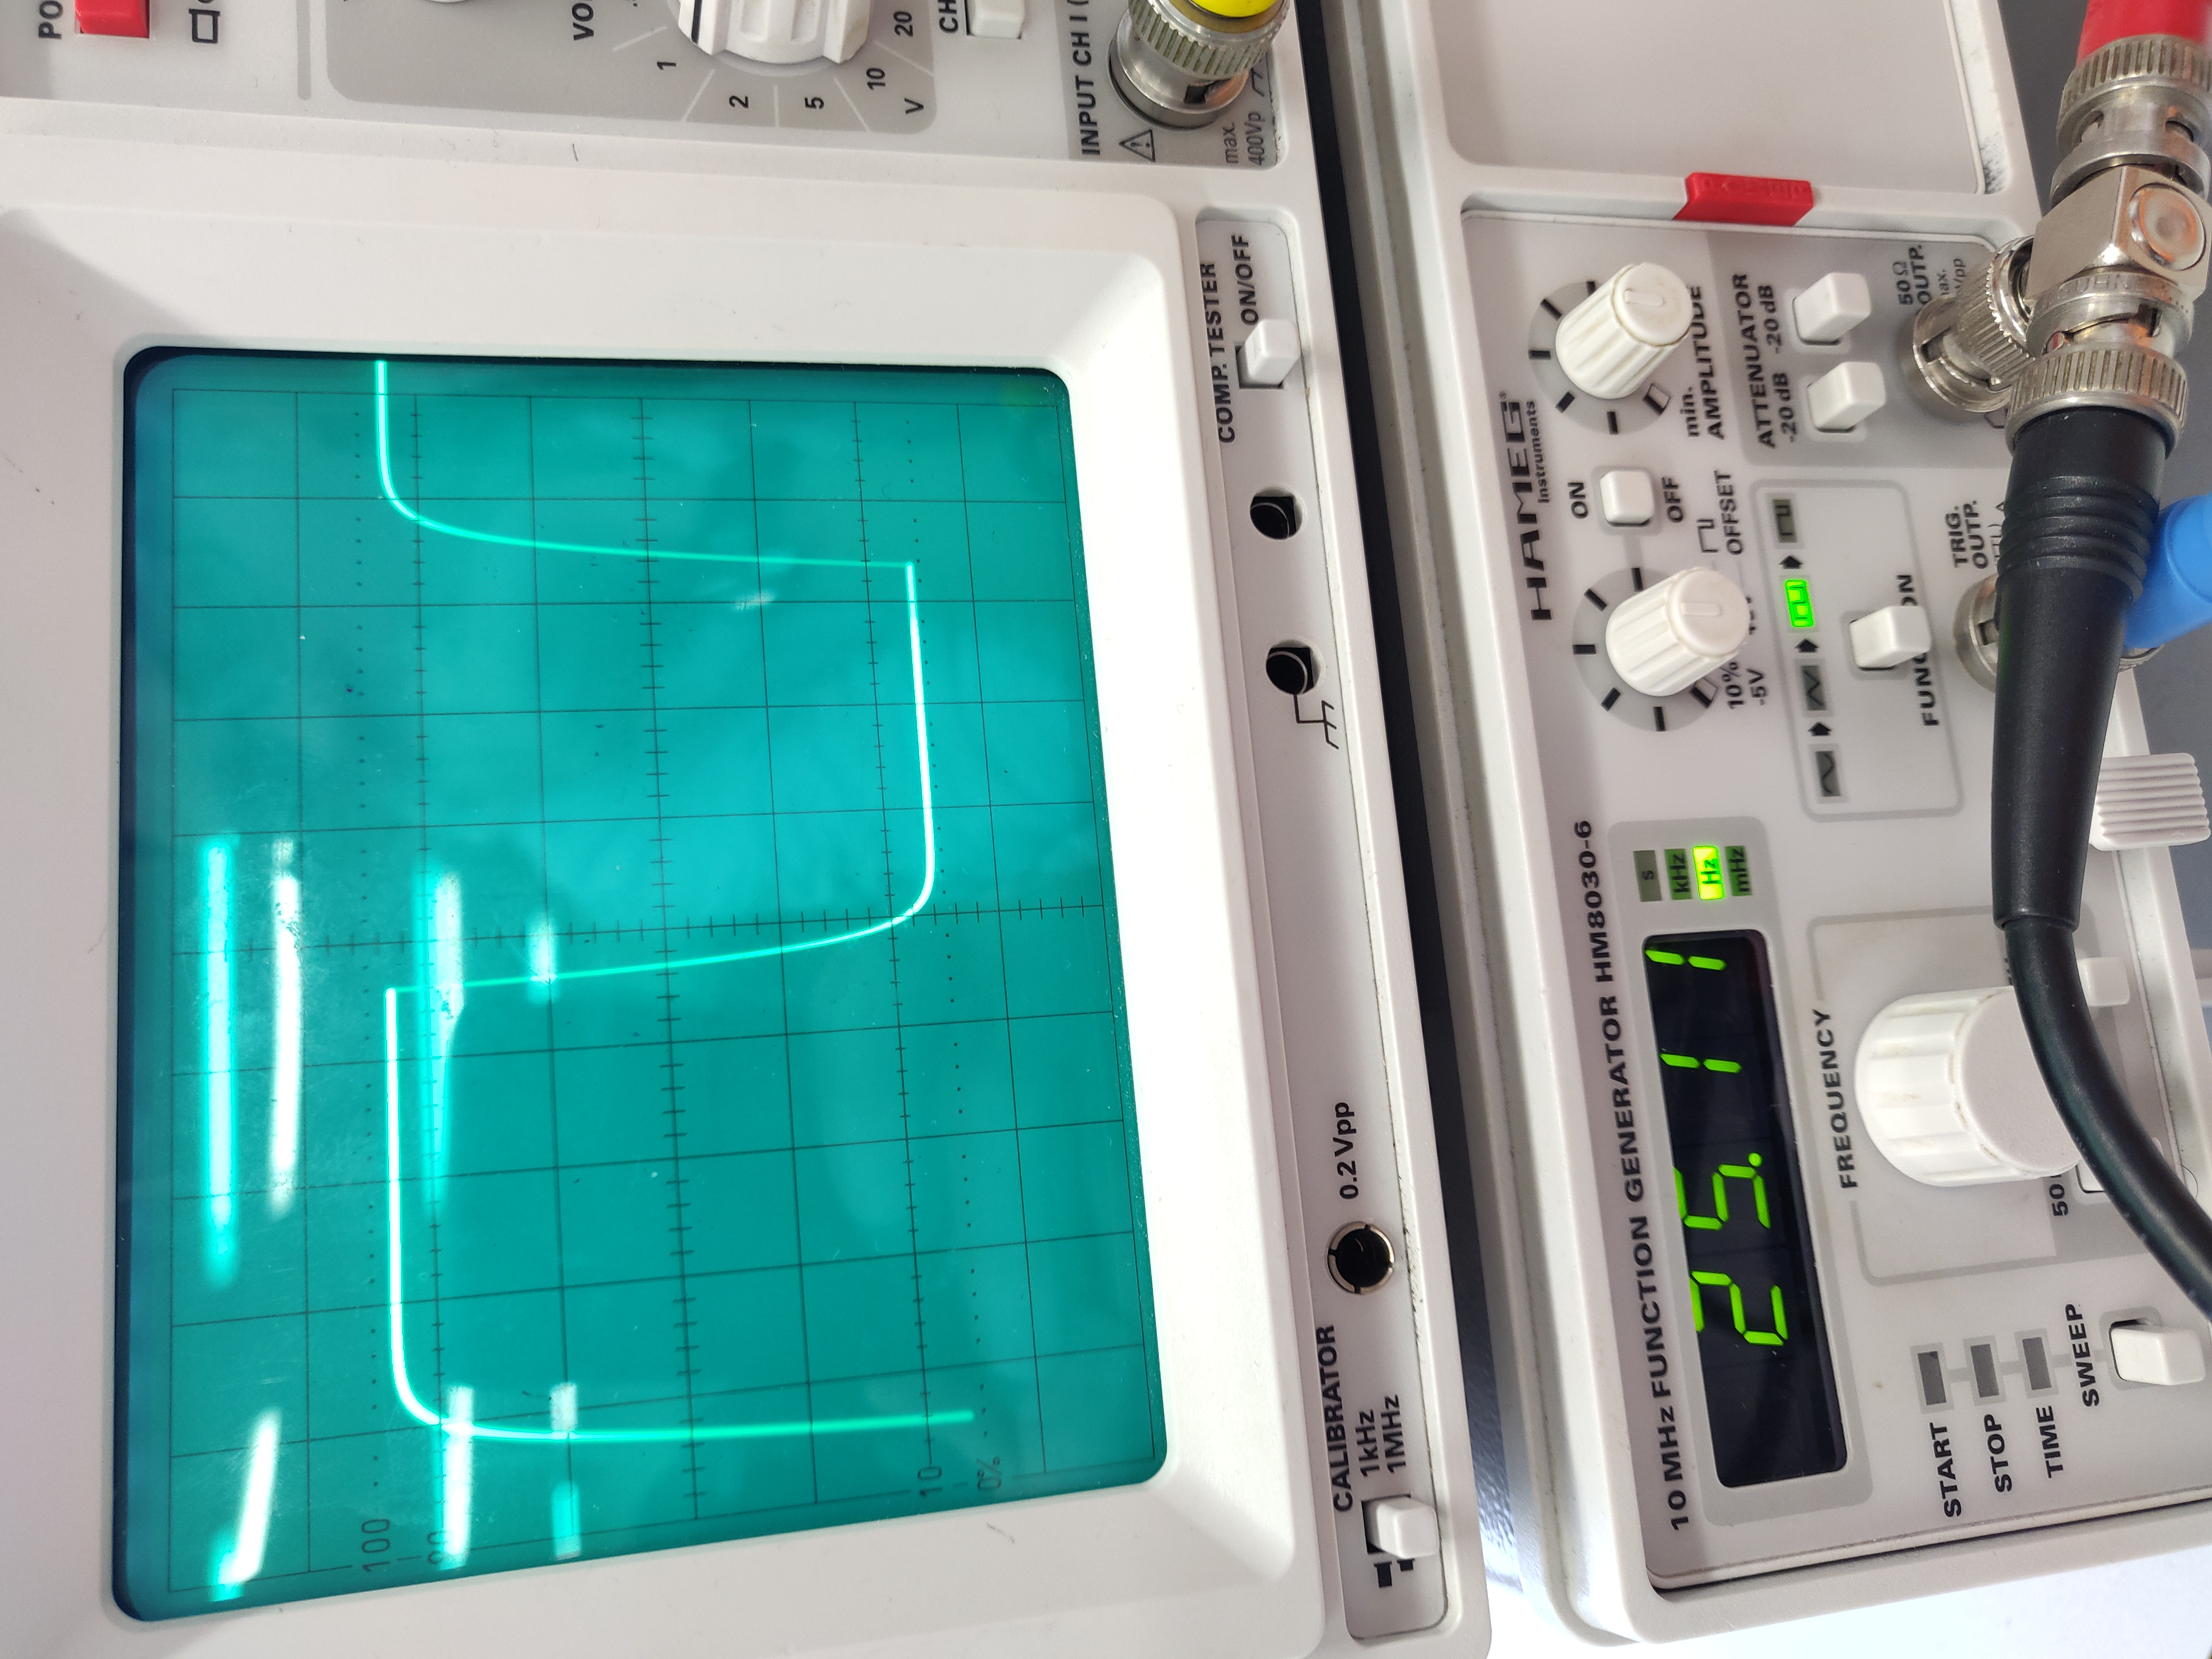
\includegraphics[height=5cm]{plots/maxLadungKond.jpg}
        \caption{Asymptotisch genäherte maximale Spannung des Kondensators.}
        \label{fig:maxU_C}
    \end{subfigure}
    \begin{subfigure}{0.48\textwidth}
        \centering
        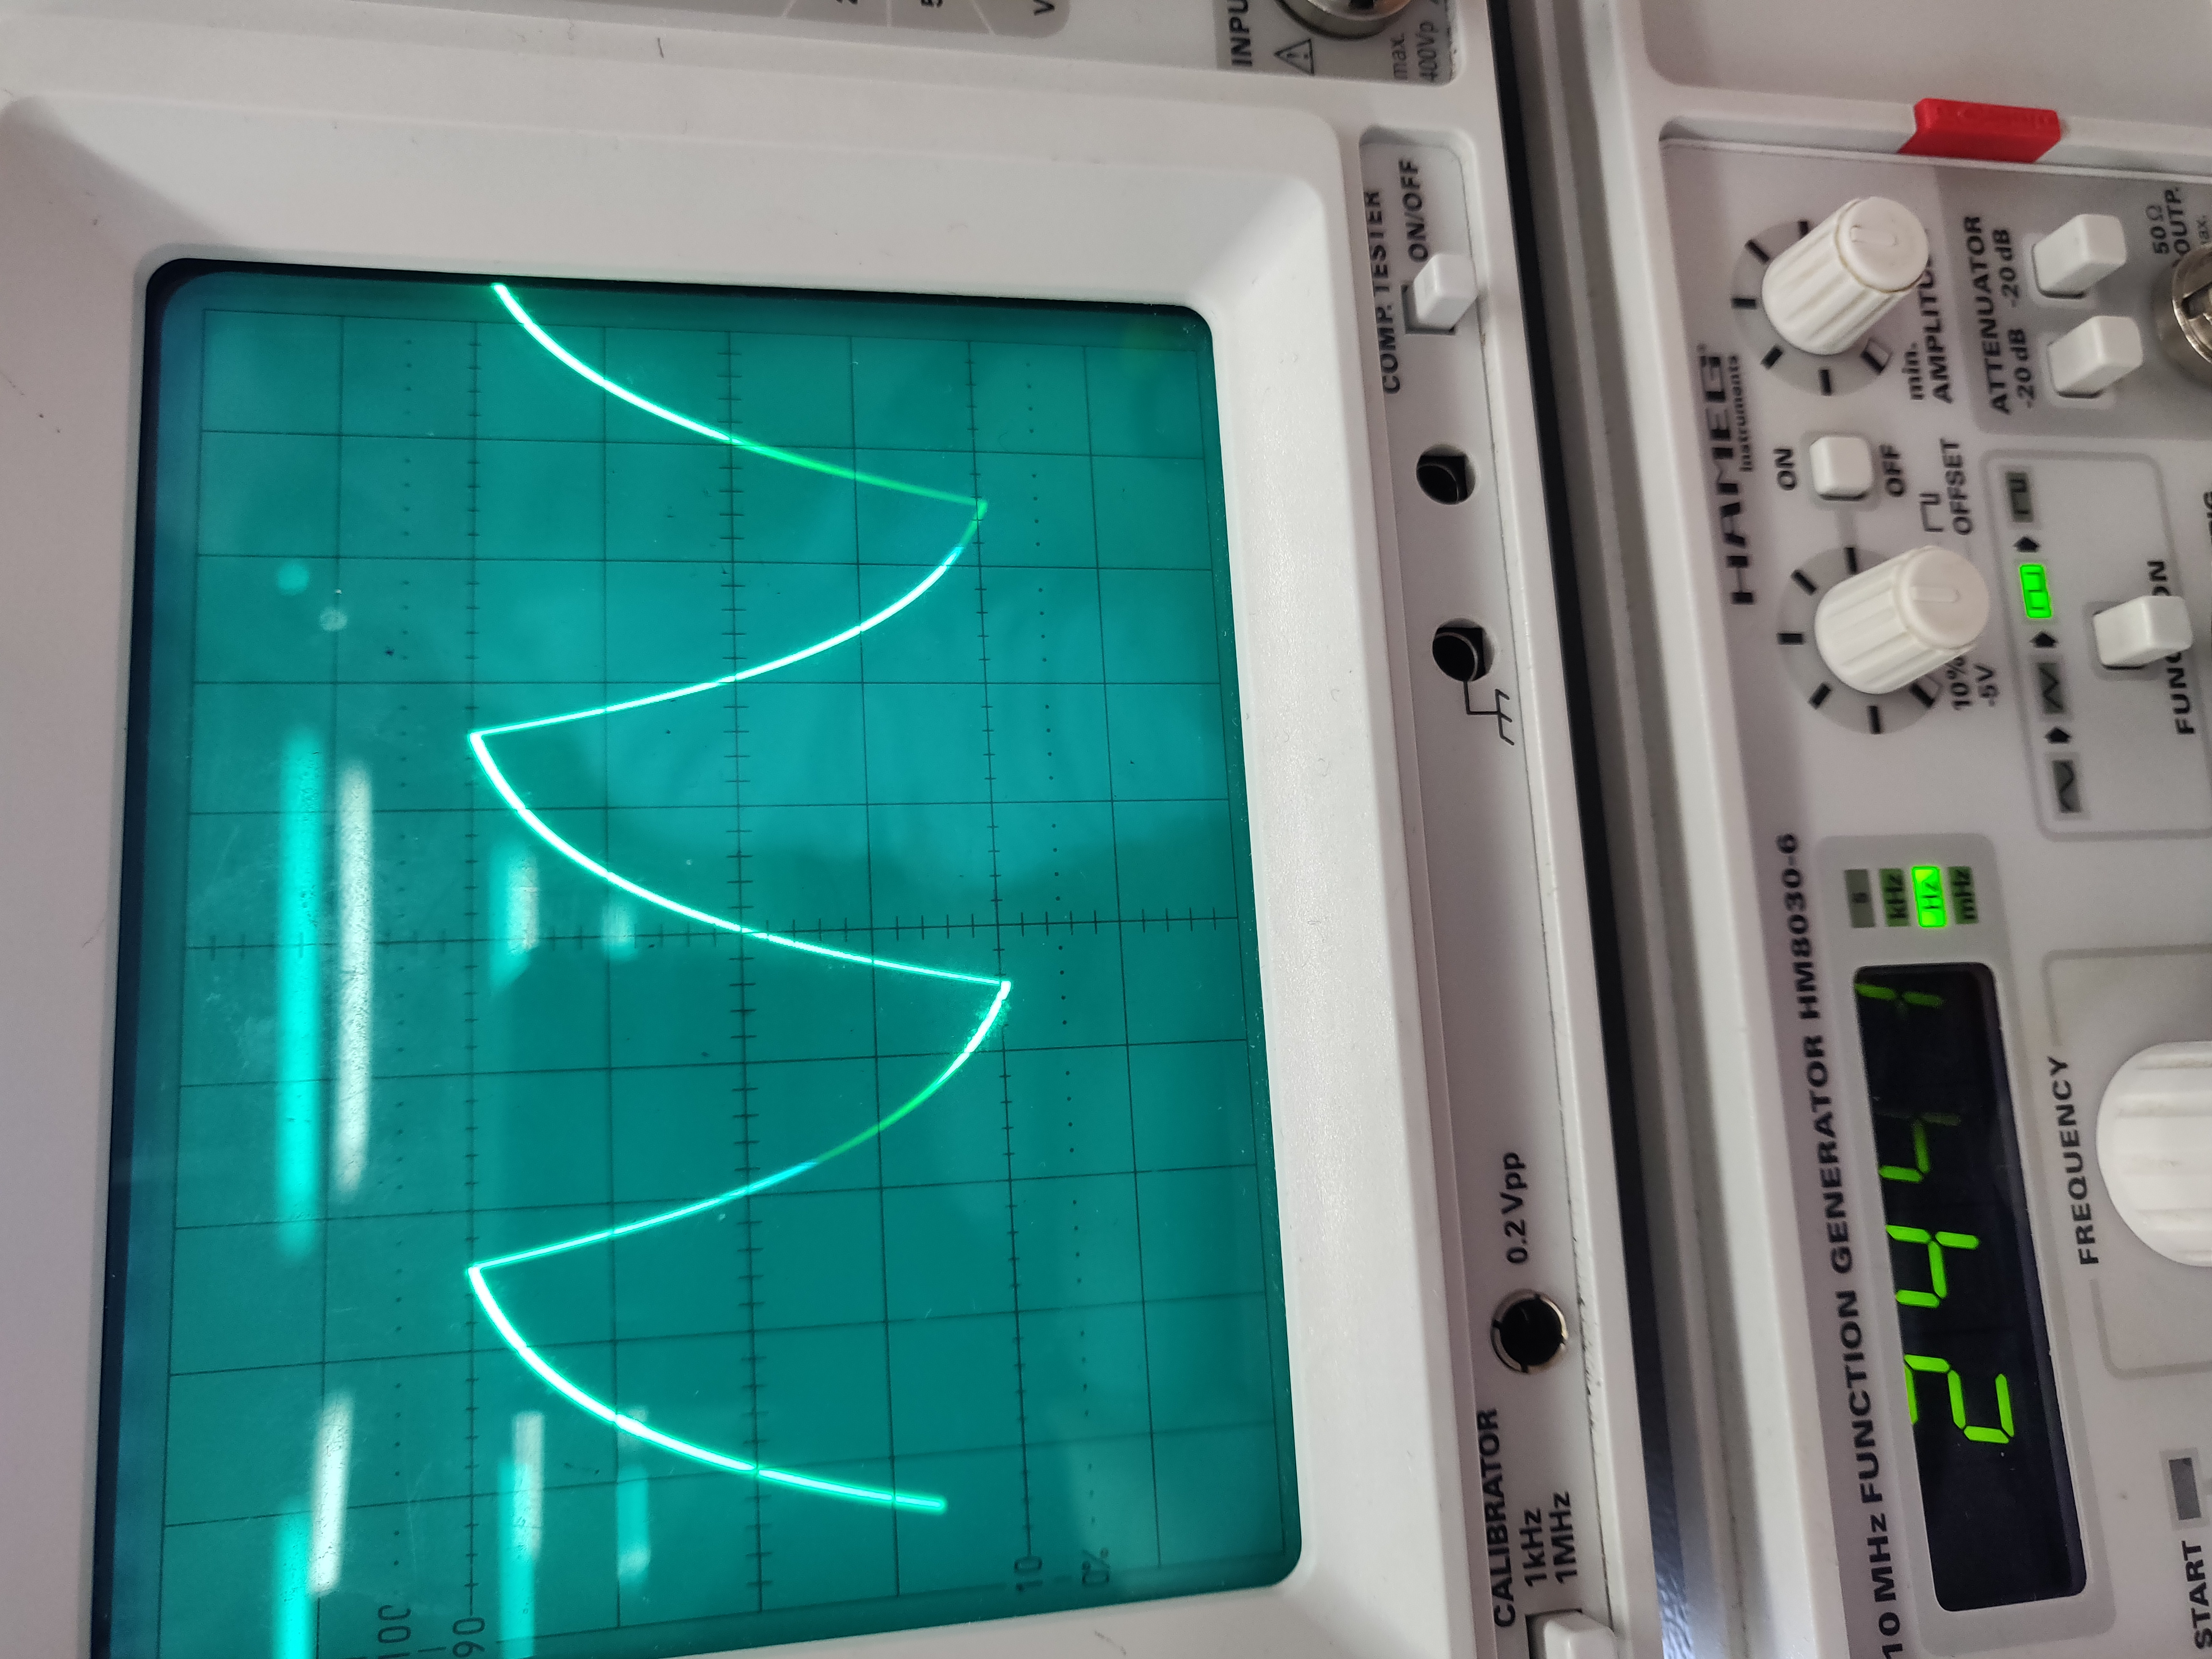
\includegraphics[height=5cm]{plots/LadungKondZacken.jpg}
        \caption{Zeitverlauf beim Auf- und Entladen.}
        \label{fig:UpAndDown}
    \end{subfigure}
    \caption{Verwendete Fotos zur Aufnahme der Messwerte.}
    \label{fig:messA}
\end{figure}

\begin{table}
    \centering
    \label{tab:Aaa}
    \caption{Messwerte zur Bestimmung der Zeitkonstante $\tau$.}
    \begin{tabular}{S[table-format=1.1] S[table-format=1.3] S[table-format=1.2]}
        \toprule
        {# Kästchen (Zeit)} & {$t\:/\:\SI{e-3}{\second}$} & {$U_C\:/\:\si{\volt}$} \\
        \midrule
        -2.4 & -2.458 & 4.35    \\
        -2.2 & -2.253 & 3.2     \\
        -2.0 & -2.048 & 2.6     \\
        -1.8 & -1.843 & 2.0     \\
        -1.6 & -1.638 & 1.6     \\
        -1.4 & -1.434 & 1.2     \\
        -1.2 & -1.229 & 0.9     \\
        -1.0 & -1.024 & 0.7     \\
        -0.8 & -0.819 & 0.55    \\
        -0.6 & -0.614 & 0.48    \\
        -0.4 & -0.410 & 0.35    \\
    \end{tabular}
\end{table}

In Tabelle \ref{tab:Aaa} sind die entsprechenden Messwerte aufgeführt, die für die folgende Ausgleichsrechnung verwendet werden. 
Wie in \ref{sub:AufUndAb} geschildert, verhält sich die Spannung eines Kondensators beim Entladen gemäß 
\begin{equation}
    U_C(t)=U_0 \exp(-\frac{1}{RC}(t-B)\:.
\end{equation}
Durch Ausgleichsrechnung mithilfe von \textit{Python 3.7.3} werd die Konstanten $A$ und $B$ von der Gerade
%Konstante B ist nötig, da die Kurve, die wir vermessen haben, ja nicht bei -2.458*10^-3 s ihr Maximum von U_0 erreicht, sondern nur 90% dessen o.ä... 
%also B ist nur zur Verschiebung der Gerade da.
\begin{equation}
    \ln{U_C(t)} = \ln{U_0} -\frac{1}{RC}(t-B) =: \ln{U_0} -A(t-B)
    \label{eqn:gerade} %U_0=4.8Volt
\end{equation} 
bestimmt. Es ergeben sich die Werte von ${A=}$ und ${B=}$. 
Die Messwerte inklusive der Geraden \eqref{eqn:gerade} sind in %hier referenz einfügen
mit passenden Achsenskalierungen aufgetragen. 

\FloatBarrier

\subsection{Frequenzabhängigkeit der Amplitude und der Phasenverschiebung}
 
%Der Generator hatte eine Spannung von 2.7 Volt

\begin{table}
    \centering
    \caption{Messung in der kleinsten Größenordnung.}
    \label{tab:BbbCcc1}
    \begin{tabular}
        \topline{S[table-format=3.2] S[table-format=1.2] S[table-format=1.3]}
        {$f\:/\:\si{\hertz}$} & {$U\:/\:\si{\volt}$} & {$\increment \phi\:/\:\symup{\pi}$} \\
        \midline
        15.25 & 2.50 & 0.035 \\
        20.50 & 2.50 & 0.037 \\
        23.25 & 2.50 & 0.050 \\
        26.65 & 2.50 & 0.047 \\
        30.20 & 2.50 & 0.051 \\
        39.50 & 2.45 & 0.067 \\
        45.40 & 2.50 & 0.077 \\
        57.25 & 2.40 & 0.092 \\
        63.50 & 2.40 & 0.098 \\
        71.40 & 2.39 & 0.112 \\
        76.20 & 2.36 & 0.120 \\
        80.40 & 2.34 & 0.127 \\
        85.60 & 2.30 & 0.132 \\
        92.60 & 2.24 & 0.143 \\
        99.90 & 2.22 & 0.151 \\
        108.2 & 2.20 & 0.157 \\
        112.1 & 2.18 & 0.169 \\
        121.7 & 2.12 & 0.179 \\
        125.0 & 2.10 & 0.187 \\
        131.3 & 2.09 & 0.193 \\
        \bottomrule
    \end{tabular}
\end{table}

\begin{table}
    \centering
    \caption{Messung in der mittleren der drei Größenordnungen.}
    \label{tab:BbbCcc2}
    \begin{tabular}
        \topline{S[table-format=3.1] S[table-format=1.2] S[table-format=1.3]}
        {$f\:/\:\si{\hertz}$} & {$U\:/\:\si{\volt}$} & {$\increment \phi\:/\:\symup{\pi}$} \\
        \midline
        184.8 & 1.82 & 0.243 \\
        216.8 & 1.68 & 0.265 \\
        250.0 & 1.58 & 0.256 \\
        284.0 & 1.42 & 0.296 \\
        310.8 & 1.35 & 0.300 \\
        347.5 & 1.23 & 0.337 \\
        378.6 & 1.16 & 0.340 \\
        414.1 & 1.08 & 0.365 \\
        442.7 & 1.01 & 0.353 \\
        476.2 & 0.97 & 0.354 \\
        507.7 & 0.92 & 0.362 \\
        531.5 & 0.88 & 0.366 \\
        556.6 & 0.85 & 0.369 \\
        599.0 & 0.80 & 0.385 \\
        \bottomrule
    \end{tabular}
\end{table}

\begin{table}
    \centering
    \caption{Messung in der größten Größenordnung.}
    \label{tab:BbbCcc3}
    \begin{tabular}
        \topline{S[table-format=4.0] S[table-format=1.2] S[table-format=1.3]}
        {$f\:/\:\si{\hertz}$} & {$U\:/\:\si{\volt}$} & {$\increment \phi\:/\:\symup{\pi}$} \\
        \midline
        699  & 0.68 & 0.400 \\
        791  & 0.60 & 0.413 \\
        892  & 0.55 & 0.415 \\
        1020 & 0.48 & 0.422 \\
        1111 & 0.43 & 0.423 \\
        1222 & 0.40 & 0.421 \\
        1333 & 0.38 & 0.429 \\
        1444 & 0.35 & 0.426 \\
        1555 & 0.32 & 0.436 \\
        1666 & 0.29 & 0.432 \\
        1777 & 0.25 & 0.446 \\
        1888 & 0.23 & 0.436 \\
        1999 & 0.22 & 0.424 \\
        2112 & 0.21 & 0.432 \\
        \midrule
        5701 & 0.07 & 0.438 \\
        \bottomrule
    \end{tabular}
\end{table}